\documentclass[a4paper,11pt]{article}
\input{/home/tof/Documents/Cozy/latex-include/preambule_doc.tex}
\input{/home/tof/Documents/Cozy/latex-include/preambule_commun.tex}
\newcommand{\showprof}{show them}  % comment this line if you don't want to see todo environment
\setlength{\fboxrule}{0.8pt}
\fancyhead[L]{\fbox{\Large{\textbf{Routage 02}}}}
\fancyhead[C]{\textbf{Routing Information Protocol}}
\newdate{madate}{10}{09}{2020}
%\fancyhead[R]{\displaydate{madate}} %\today
%\fancyhead[R]{Seconde - SNT}
%\fancyhead[R]{Première - NSI}
\fancyhead[R]{Terminale - NSI}
\fancyfoot[L]{\vspace{1mm}Christophe Viroulaud}
\AtEndDocument{\label{lastpage}}
\fancyfoot[C]{\textbf{Page \thepage/\pageref{lastpage}}}
\fancyfoot[R]{\includegraphics[width=2cm,align=t]{/home/tof/Documents/Cozy/latex-include/cc.png}}

\begin{document}
\section{Problématique}
Le nombre de routeurs est généralement trop grand pour envisager construire les tables de routage à la main. En effet une modification du réseau (panne, nouvel élément\dots) implique de recalculer toutes les routes.
\begin{center}
    \framebox{Comment construire les tables de routage dynamiquement?}
\end{center}
\section{Protocole de routage}
\subsection{Principe}
En plus des paquets, les routeurs s'échangent des informations sur la topologie du réseau. 
\begin{aretenir}[]
    Chaque routeur applique les mêmes règles de communication et de description: c'est le \textbf{protocole de routage}.
\end{aretenir}
\subsection{Protocole RIP - Routing Information Protocol}
À intervalle régulier (30 secondes par défaut), chaque routeur transmet à ses voisins les adresses de ses propres voisins et celles qu'il a reçues par d'autres routeurs. Il précise également la distance (en \emph{nombre de sauts}) pour atteindre une machine donnée.
\begin{aretenir}[]
Le protocole RIP échange des \textbf{vecteurs de distance} (couple adresse/distance) avec ses routeurs voisins.
\end{aretenir}
L'objectif du protocole RIP est de minimiser le nombre de sauts pour atteindre la destination. Il construit et modifie sa table de routage en fonction des informations qu'il reçoit.
\section{Table de routage}
Chaque ligne de la table de routage contient quatre informations:
\begin{itemize}
    \item la \emph{destination} sous la forme adresse de sous-réseau/masque,
    \item la \emph{passerelle} est l'adresse IP du prochain routeur à traverser,
    \item l'\emph{interface} réseau à utiliser pour rejoindre la passerelle,
    \item la \emph{distance} vers la destination.
\end{itemize}
\begin{center}
    \centering
    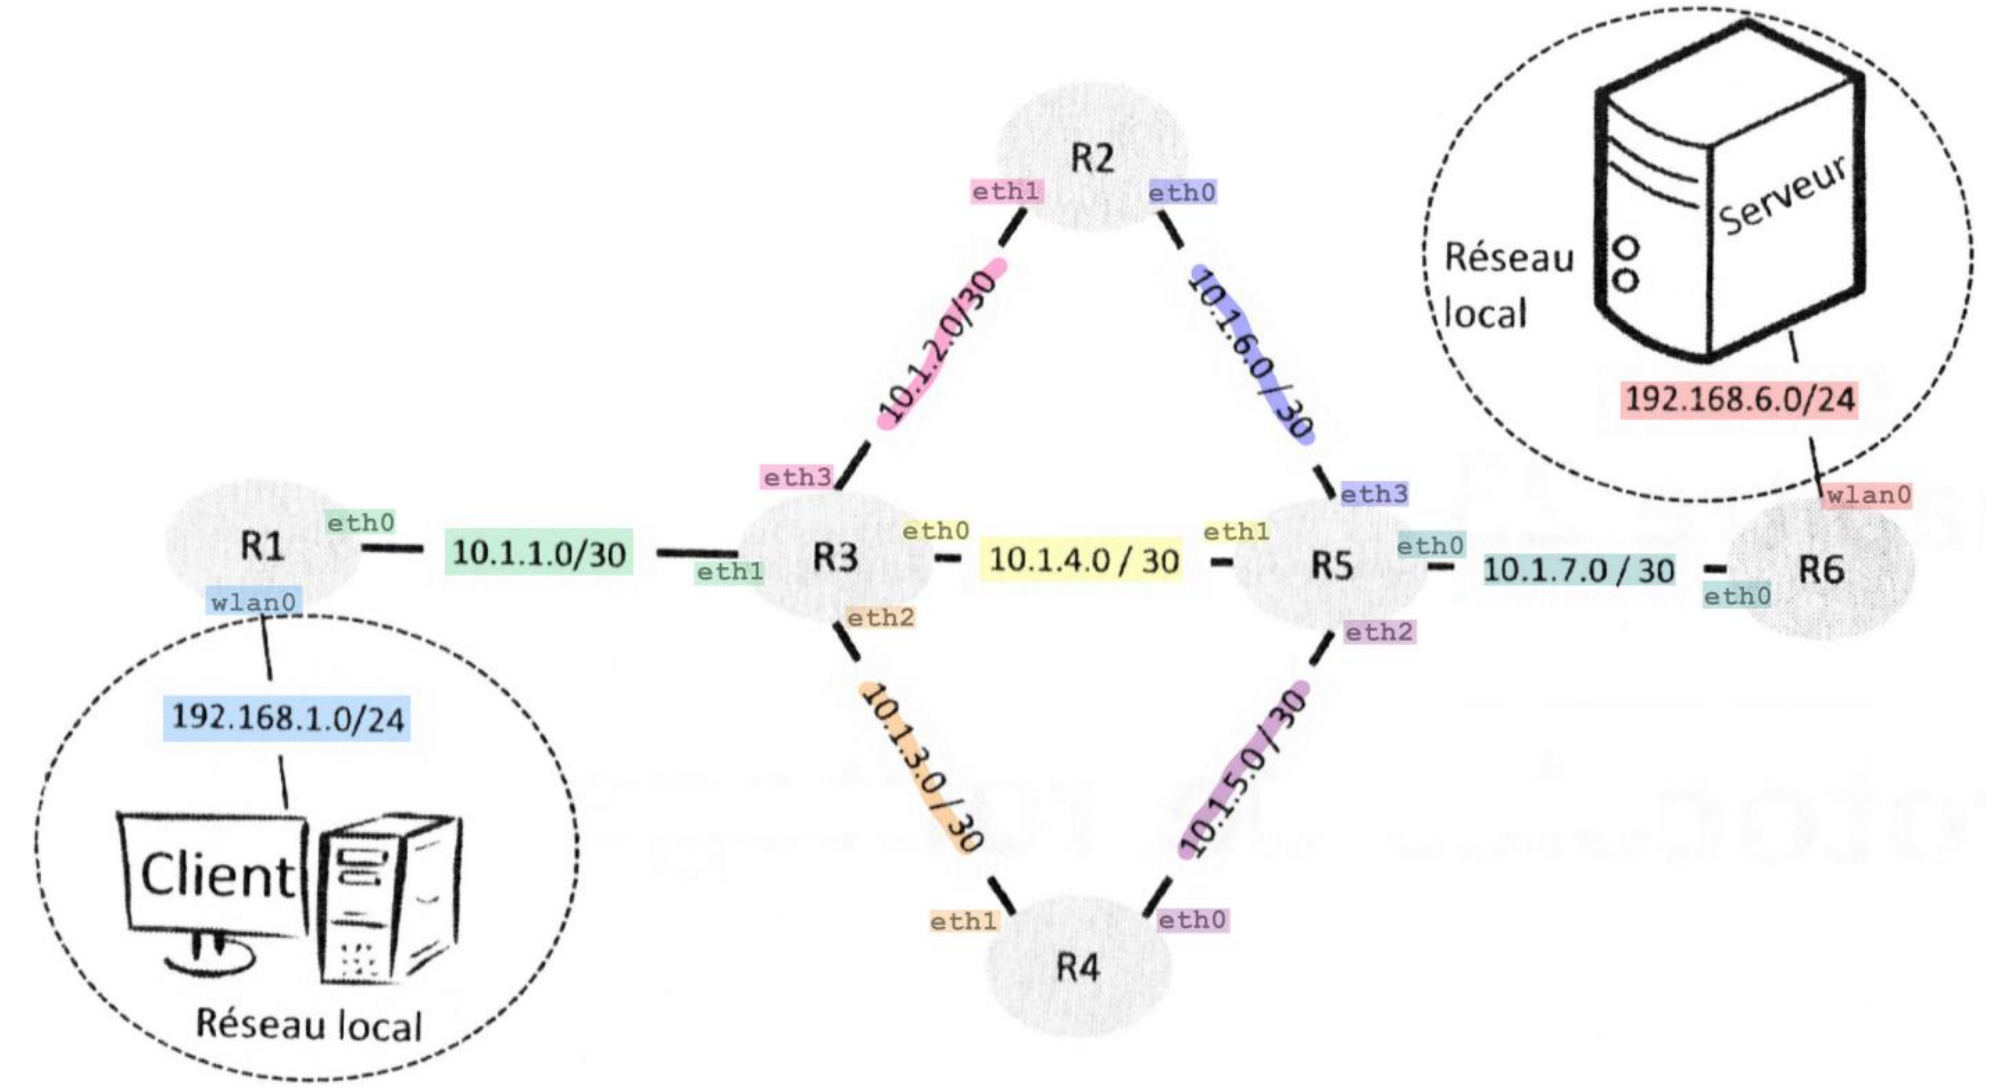
\includegraphics[width=16cm]{ressources/reseau.png}
    \captionof{figure}{Topologie du réseau}
    \label{reseau}
\end{center}
\paragraph{Lors de la phase d'initialisation} (allumage de l'appareil), le routeur récupère les informations de ses voisins immédiats.
\begin{center}
    \begin{tabular}{|*{4}{c|}}
        \hline
        destination & passerelle & interface & distance \\
        \hline
        10.1.1.0/30 & & eth0 & 1\\
        \hline
        192.168.1.0/24 & & wlan0 & 1\\
        \hline
    \end{tabular}
    \captionof{table}{Table de routage de R1}
\end{center}
\begin{aretenir}[Remarque]
La passerelle est vide quand l'adresse de destination est celle du routeur voisin.
\end{aretenir}
\begin{activite}
Construire la table de routage du routeur R3 lors de la phase d'initialisation.
\end{activite}
\paragraph{Les routeurs effectuent ensuite des demandes RIP.} Lorsqu'un routeur reçoit une demande il accuse réception en renvoyant sa table de routage.

Avec la réponse de son voisin, le routeur a quatre possibilités :
\begin{itemize}
    \item Il découvre une nouvelle route vers un sous-réseau qui lui était jusque-là inconnu : il l’inscrit dans sa table.
    \item Il découvre une route plus courte vers un sous-réseau connu mais passant par un autre routeur : il efface l’ancienne route de sa table et inscrit la nouvelle.
    \item Il reçoit une nouvelle route plus longue : il l’ignore.
    \item Il reçoit une route existante, mais plus longue, vers un routeur passant par le même voisin. Cela veut dire qu’un problème est apparu sur son ancienne route. Il met donc à jour sa table avec cette nouvelle route.
\end{itemize}
\begin{aretenir}[Remarque]
    Lorsqu’un routeur reçoit une route, il augmente la distance associée à cette route de 1 pour prendre en compte que les paquets devront passer par
    lui.
\end{aretenir}
\begin{center}
    \begin{tabular}{|*{4}{c|}}
        \hline
        destination & passerelle & interface & distance \\
        \hline
        10.1.1.0/30 & & eth0 & 1\\
        \hline
        192.168.1.0/24 & & wlan0 & 1\\
        \hline
        10.1.2.0/30 & R3 & eth0 & 2 \\
        \hline
        10.1.3.0/30 & R3 & eth0 & 2 \\
        \hline
        10.1.4.0/30 & R3 & eth0 & 2 \\
        \hline
    \end{tabular}
    \captionof{table}{Table de routage de R1 après son échange avec R3}
\end{center}
\begin{activite}
\begin{enumerate}
    \item Construire la table de routage de R3 après son échange avec R1.
    \item Construire la table de routage de R5 lors de la phase d'initialisation.
    \item Construire ensuite la table de routage de R3 après son échange avec R5.
\end{enumerate}
\end{activite}
\section{Gestion des pannes}
Le protocole est conçu pour détecter les pannes ou les dyfonctionnements (boucle de routage). Plusieurs mécanismes sont mis en place:
\begin{itemize}
    \item \textbf{15 sauts maximum:} au-delà la route est oubliée.
    \item \textbf{split horizon:} toutes les routes accessibles via une certaine interface ne doivent pas être incluses dans une mise à jour sortant par cette même interface.
    \item \textbf{hold down:} lorsqu'un routeur prend connaissance de l'indisponibilité d'une route vers un sous-réseau, il doit ignorer toute information concernant un chemin vers ce sous réseau pendant une durée égale au \emph{temporisateur (hold down)}. 
\end{itemize}
\begin{aretenir}[Remarque]
La limite de 15 sauts ne permet pas d'utiliser ce protocole pour de grands réseaux.
\end{aretenir}
\end{document}